% begin module inverse-function-equations
\begin{frame}
\[
\alert<handout:0| 4>{f^{-1}(y) = x} \qquad \Leftrightarrow \qquad \alert<handout:0| 3>{f(x) = y} .
\]
\uncover<2->{Therefore
\[
(f^{-1}\circ f)(x) = f^{-1}(\alert<handout:0| 3>{f(x)}) = \uncover<3->{\alert<handout:0| 4>{f^{-1}(\alert<handout:0| 3-4>{y})}} \uncover<4->{\alert<handout:0| 4>{ = x}.}
\]
}
\uncover<5->{
\psset{xunit=0.75cm, yunit=0.75cm}
\begin{pspicture}(-4, -2.5)(13,2.5) 
\footnotesize
\psframe*[linecolor=white](-5,-5)(5,5) 
\rput[r] (-3.1, 0){$x$}
\psline[linewidth=3pt]{->}(-3,0)(-2.25,0)

\rput(0.25,0){
\psMachine{$f$}{red}
}
\rput (4, 0){$f(x)$}
\psline[linewidth=3pt]{->}(2.75,0)(3.5,0)
\psline[linewidth=3pt]{->}(4.5,0)(5.25,0)
\rput(7.75,0){
\psMachine{$f^{-1}$}{blue}
}
\rput (11.75, 0){$x$}
\psline[linewidth=3pt]{->}(10.25,0)(11,0)
\end{pspicture} 
%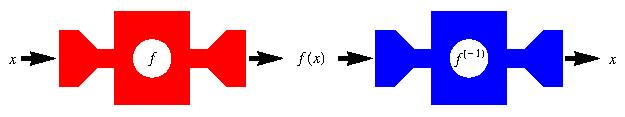
\includegraphics[height=2cm]{inverse-functions/pictures/07-01-machinesb.pdf}%
}
\uncover<6->{
Switch the roles of $x$ and $y$:
\[
\alert<handout:0| 8>{f^{-1}(x) = y} \qquad \Leftrightarrow \qquad \alert<handout:0| 9>{f(y) = x} .
\]
}
\uncover<7->{Therefore
\[
(f\circ f^{-1})(x) = f(\alert<handout:0| 8>{f^{-1}(x)}) = \uncover<8->{\alert<handout:0| 9>{f(\alert<handout:0| 8-9>{y})}} \uncover<9->{\alert<handout:0| 9>{ = x}.}
\]
}
\uncover<10->{
\psset{xunit=0.75cm, yunit=0.75cm}
\begin{pspicture}(-4, -2.5)(13,2.5) 
\footnotesize
\psframe*[linecolor=white](-5,-5)(5,5) 
\rput[r] (-3.1, 0){$x$}
\psline[linewidth=3pt]{->}(-3,0)(-2.25,0)

\rput(0.25,0){
\psMachine{$f^{-1}$}{red}
}
\rput (4, 0){ $f^{-1}(x)$}
\psline[linewidth=3pt]{->}(2.75,0)(3.4,0)
\psline[linewidth=3pt]{->}(4.7,0)(5.25,0)
\rput(7.75,0){
\psMachine{$f$}{blue}
}
\rput (11.75, 0){$x$}
\psline[linewidth=3pt]{->}(10.25,0)(11,0)
\end{pspicture} 
%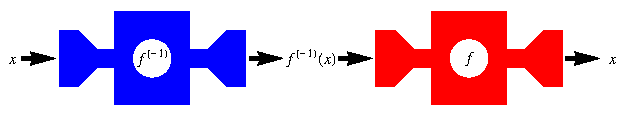
\includegraphics[height=2cm]{inverse-functions/pictures/07-01-machinesa.pdf}%
}
\end{frame}
% end module inverse-function-equations
